\documentclass[UTF8, a4paper, fontset=none]{article}
\usepackage{amsfonts}
\usepackage{amsmath}
\usepackage{amssymb}
\usepackage{amsthm}
\usepackage{courier}
\usepackage{ctex}
\usepackage{geometry}
\usepackage{graphicx}
\usepackage{hyperref}
% \usepackage{listings}
\geometry{left=2.5cm,right=2.5cm,top=2.5cm,bottom=2.5cm}
\ctexset{fontset=fandol}

\begin{document}

\title{手掌活体检测——实验报告}
\author{马栩杰, 严靖凯, 黄秀峰, 邢成 \footnote{马栩杰,2014011085,无43班;严靖凯,2014011192,无46班;黄秀峰,2014011193,无46班;邢成,2014011167,无46班}}
\maketitle

\section{背景介绍}

目前随着机器学习、模式识别领域的迅速发展,诸如人脸检测、指纹检测、掌纹检测等基于生物特征的个体识别方式正逐渐取得广泛的应用。与此同时,正如2017年央视“3·15”晚会中所提及的,针对这些特征的活体检测方法在当前越来越称为问题的核心之一。只有当识别系统具备了活体检测的能力,才能避免攻击者通过事先获取的静态信息进行直接攻击,从而大大增强识别系统的鲁棒性。

具体到掌纹时变与手掌活体的检测问题中,我们需要验证检测系统中拍摄到的手掌是否为活体。关于这方面的文章目前很少,因此我们也借鉴了部分人脸活体检测、指纹活体检测中的思路。

\section{系统设计}

\begin{figure}
    \centering
    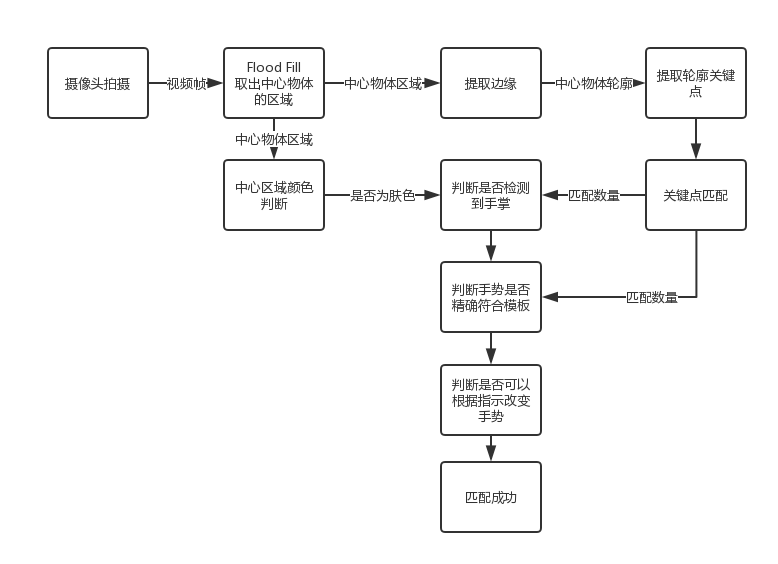
\includegraphics[width=0.9\textwidth]{./system.png}
    \caption{系统整体结构}
    \label{system}
\end{figure}

手掌活体检测系统的整体结构如图 \ref{system} 所示。

对于摄像头捕获到的单帧画面,首先提取画面中心的物体,然后取该物体的轮廓,从轮廓上取出若干个显著的峰/谷点作为关键点,将关键点与预先定义的手势模板中的关键点进行匹配。

判断画面中心物体是否为手掌的依据是关键点匹配成功的点数 N 大于阈值 $ th_{num, 1} $ (检测到点与模板关键点 \emph{基本匹配} 的匹配点数阈值), 并且中心物体的平均颜色接近肤色。

在此基础上,如果匹配成功的关键点数量大于 $ th_{num, 2} $ (检测到点与模板关键点 \emph{完全匹配} 的匹配点数阈值),则认为检测到物体的关键点与当前的模板完全匹配,认为用户已经做出模板指示的手势,此时更换模板,并且提示用户做出下一个动作。

当用户连续完成若干个指示时,就认为用户通过了活体检测。

\section{模块设计}

\subsection{中心物体提取}

中心物体提取使用 Flood Fill 算法。

系统假设进行活体检测时,用户的手掌位于画面中央。于是取画面的中心点为起始点,以 4 邻域内像素的颜色变化是否小于阈值做为 Flood Fill 是否继续进行的判断依据,执行 Flood Fill 算法,提取出画面中心颜色相近的一块区域。

此时提取出的中心区域边缘有很多不平整的部分,先后执行形态学开运算和闭运算使得提取出的物体形状上更光滑。

\subsection{边缘关键点提取}

提取出中心物体之后,取出其轮廓点,并在轮廓点中选取关键点。

\begin{figure}
    \centering
    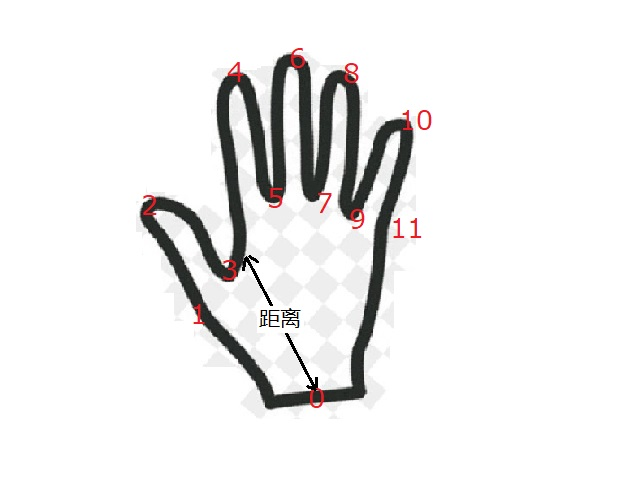
\includegraphics[width=0.6\textwidth]{./hand.jpg}
    \caption{关键点定义}
    \label{hand}
\end{figure}

关键点的定义如图 \ref{hand} 所示。

提取出中心物体的轮廓之后,按顺序计算轮廓上点到预定义模板关键点 0(手掌根部)的欧式距离。理想情况下,该距离函数至少会出现 5 个显著的峰值(指尖)和 4 个显著的谷值(指根)。取出距离函数中位于峰值和谷值位置的点作为轮廓上的关键点。此时对取出的关键点数量不做约束。

\subsection{关键点匹配}

在提取出关键点之后,将提取出的关键点和模板关键点进行配对。对检测到的关键点和模板关键点进行一次二分图匹配,将模板关键点与距离其最近的检测到的关键点配对。如果配对后的两点的欧式距离小于阈值,则认为该关键点对匹配成功。最终匹配出的关键点对应该不超过 9 个(图 \ref{hand} 中的关键点 2 到 10)。

\section{实验}

    \subsection{使用流程}

    \subsection{模拟攻击}

\section{系统评价}



\end{document}
